\documentclass[12pt]{report}
\usepackage[utf8]{inputenc}
\usepackage[russian]{babel}
%\usepackage[14pt]{extsizes}
\usepackage{listings}

% Для листинга кода:
\lstset{ %
language=go,                 % выбор языка для подсветки 
basicstyle=\small\sffamily, % размер и начертание шрифта для подсветки кода
numbers=left,               % где поставить нумерацию строк (слева\справа)
numberstyle=\tiny,           % размер шрифта для номеров строк
stepnumber=1,                   % размер шага между двумя номерами строк
numbersep=5pt,                % как далеко отстоят номера строк от подсвечиваемого кода
showspaces=false,            % показывать или нет пробелы специальными отступами
showstringspaces=false,      % показывать или нет пробелы в строках
showtabs=false,             % показывать или нет табуляцию в строках            
tabsize=2,                 % размер табуляции по умолчанию равен 2 пробелам
captionpos=t,              % позиция заголовка вверху [t] или внизу [b] 
breaklines=true,           % автоматически переносить строки (да\нет)
breakatwhitespace=false, % переносить строки только если есть пробел
escapeinside={\#*}{*)}   % если нужно добавить комментарии в коде
}

% Для измененных титулов глав:
\usepackage{titlesec, blindtext, color} % подключаем нужные пакеты
\definecolor{gray75}{gray}{0.75} % определяем цвет
\newcommand{\hsp}{\hspace{20pt}} % длина линии в 20pt
% titleformat определяет стиль
\titleformat{\chapter}[hang]{\Huge\bfseries}{\thechapter\hsp\textcolor{gray75}{|}\hsp}{0pt}{\Huge\bfseries}

\usepackage{amsmath}
\usepackage{mathptmx}
% plot
\usepackage{pgfplots}
\usepackage{filecontents}
\usepackage{amsmath}
\usepackage{tikz,pgfplots}
\usetikzlibrary{datavisualization}
\usetikzlibrary{datavisualization.formats.functions}

\usepackage{geometry}
\geometry{verbose, a4paper,tmargin=2cm, bmargin=2cm, rmargin=1.5cm, lmargin = 3cm}

\usepackage{graphicx}
\graphicspath{{src/}}
\DeclareGraphicsExtensions{.pdf,.png,.jpg}

\begin{document}
%\def\chaptername{} % убирает "Глава"
\begin{titlepage}
	\centering
	{\scshape\LARGE МГТУ им. Баумана \par}
	\vspace{3cm}
	{\scshape\Large Рубежный контроль №2\par}
	\vspace{0.5cm}	
	{\scshape\Large По курсу: "Анализ алгоритмов"\par}
	\vspace{1.5cm}
	{\huge\bfseries Регулярные выражения \par}
	\vspace{2cm}
	\Large Работу выполнил: Мокеев Даниил, ИУ7-54\par
	\vspace{0.5cm}
	\Large Преподаватели:  Волкова Л.Л., Строганов Ю.В.\par

	\vfill
	\large \textit {Москва, 2019} \par
\end{titlepage}

\tableofcontents

\newpage
\chapter*{Введение}
\addcontentsline{toc}{chapter}{Введение}

Цель работы: изучение возможности регулярных выражений. Реализация поиска по тексу при использовании регулярных выражений и конечного автомата.
В ходе рубежного контроля предстоит:
\begin{itemize}
	\item Изучить регулярные выражения; 
	\item реализовать поиск по тексту всех вхожедний цикла for с помощью регулярных выражений и конечного автомата.
\end{itemize}

\chapter{Аналитическая часть}
Регулярные выражения (англ. regular expressions) — формальный язык поиска и осуществления манипуляций с подстроками в тексте, основанный на использовании метасимволов (символов-джокеров, англ. wildcard characters). Для поиска используется строка-образец (англ. pattern, по-русски её часто называют «шаблоном», «маской»), состоящая из символов и метасимволов и задающая правило поиска. Для манипуляций с текстом дополнительно задаётся строка замены, которая также может содержать в себе специальные символы.


\section{Использование регулярных выражений}
Регулярные выражения используются некоторыми текстовыми редакторами и утилитами для поиска и подстановки текста. Например, при помощи регулярных выражений можно задать шаблоны, позволяющие:
\begin{itemize}
	\item найти все последовательности символов «кот» в любом контексте, как то: «кот», «котлета», «терракотовый»;
	\item найти отдельно стоящее слово «кот» и заменить его на «кошка»;
	\item найти слово «кот», которому предшествует слово «персидский» или «чеширский»;
	\item убрать из текста все предложения, в которых упоминается слово кот или кошка.
\end{itemize}
Регулярные выражения позволяют задавать и гораздо более сложные шаблоны поиска или замены.

Результатом работы с регулярным выражением может быть:
\begin{itemize}
	\item проверка наличия искомого образца в заданном тексте;
	\item определение подстроки текста, которая сопоставляется образцу;
	\item определение групп символов, соответствующих отдельным частям образца.
\end{itemize}
Если регулярное выражение используется для замены текста, то результатом работы будет новая текстовая строка, представляющая из себя исходный текст, из которого удалены найденные подстроки (сопоставленные образцу), а вместо них подставлены строки замены (возможно, модифицированные запомненными при разборе группами символов из исходного текста). Частным случаем модификации текста является удаление всех вхождений найденного образца — для чего строка замены указывается пустой.
\section{Регулярные выражения в теории формальных языков}
Регулярные выражения состоят из констант и операторов, которые определяют множества строк и множества операций на них соответственно. Определены следующие константы:
\begin{itemize}
\item (пустое множество) $\emptyset$.
\item (пустая строка) $\epsilon$ обозначает строку, не содержащую ни одного символа; эквивалентно \"".
\item (символьный литерал) "a", где a — символ используемого алфавита.
\item (множество) из символов, либо из других множеств.
и следующие операции:
\end{itemize}
\begin{itemize}
	\item (сцепление, конкатенация) RS обозначает множество ${\alpha\beta | \alpha \in R  \& \beta \in S}$. Например, \{"boy", "girl"\}\{"friend", "cott"\} = \{"boyfriend", "girlfriend", "boycott", "girlcott"\}.
	\item(дизъюнкция, чередование) $R|S$ обозначает объединение R и S.
	
	 Например, \{"ab", "c"\}|\{"ab", "d", "ef"\} = \{"ab", "c", "d", "ef"\}.
	\item(замыкание Клини, звезда Клини) R* обозначает минимальное надмножество множества R, которое содержит $\epsilon$ и замкнуто относительно конкатенации. Это есть множество всех строк, полученных конкатенацией нуля или более строк из R.
	
	 Например, \{"Run", "Forrest"\}* = \{$\epsilon$, "Run", "Forrest", "RunRun", "RunForrest", "ForrestRun",
	 
	  "ForrestForrest", "RunRunRun",
	
	 "RunRunForrest", "RunForrestRun", \}.
	\item Регулярные выражения, входящие в современные языки программирования (в частности, PCRE), имеют больше возможностей, чем то, что называется регулярными выражениями в теории формальных языков; в частности, в них есть нумерованные обратные ссылки. Это позволяет им разбирать строки, описываемые не только регулярными грамматиками, но и более сложными, в частности, контекстно-свободными грамматиками.
\end{itemize}
\section{Вывод}
Были рассмотренны регулярныные выражения и их обоснование в теории формальных языков.

\chapter{Конструкторская часть}
\section{Требования к программе}
\textbf{Требования к вводу:}
\begin{itemize}
	\item На вход подается код программы на языке golang в формате .txt;
	\item количество вхождений цикла for в строке не больше 1.
\end{itemize}
\textbf{Требования к программе:}
\begin{itemize}
	\item Программа выводит все строки, в которых встречается вхождения условия цикла for;
	\item программа должна выводить строки с циклом for даже если его условие некорректно.
\end{itemize}
\section{Матрица переходов}
В этом разделе будет рассмотрена матрица переходов конечного автомата (Рис. \ref{fig:avt})

\begin{figure}[h]
	\centering{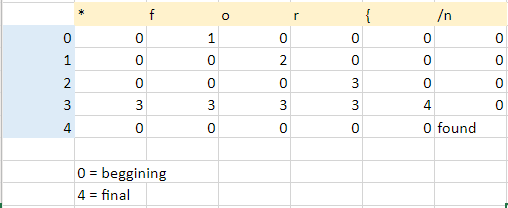
\includegraphics[scale = 1.3]{table.png}}
	\caption{Таблица переходов состояний}
	\label{fig:avt}
\end{figure}

\section{Вывод}
В данном разделе была рассмотрена матрица переходов реализованного автомата и требования к работе программы.

\chapter{Технологическая часть}
\section{Выбор ЯП}
Я выбрал в качестве языка программирования Golang, потому как он достаточно удобен.

\section{Листинг кода алгоритмов}
В данном разделе будет представлен листинги кода поиска с помощью регулярных выражений (\ref{RegExp}), с помощью конечного автомата(\ref{Avt})
\begin{lstlisting}[label=RegExp,caption = Использование регулярных выражений]
func get_fors(name_file string) []string{
	answer:=make([]string, 0)
	for_pattern:="(for).*\\{+"
	get_for, _ := regexp.Compile(for_pattern)
	file, err := os.Open(name_file)
	if err != nil{
		fmt.Println(err)
		os.Exit(1)
	}
	defer file.Close()
	reader := bufio.NewReader(file)
	for {
		str, err := reader.ReadString('\n')
		if err == io.EOF{
		break}
		if (get_for.MatchString(str)){
			answer = append(answer, get_for.FindString(str))
		}
	}
	return answer
}
\end{lstlisting}

\begin{lstlisting}[label=Avt,caption=Использование конечного автомата]
type avt struct {
	state int
	trans map[key]int
}	

type key struct{
	symb byte
	state int
}

func new_avt() *avt{
	avt := new(avt)
	avt.state  = 0
	avt.trans = make(map[key]int)
	avt.trans[key{symb: byte('f'), state: 0}] = 1
	avt.trans[key{symb: byte('f'), state: 1}] = 0
	avt.trans[key{symb: byte('f'), state: 2}] = 0
	avt.trans[key{symb: byte('f'), state: 3}] = 3
	avt.trans[key{symb: byte('f'), state: 4}] = 0
	
	avt.trans[key{symb: byte('o'), state: 0}] = 0
	avt.trans[key{symb: byte('o'), state: 1}] = 2
	avt.trans[key{symb: byte('o'), state: 2}] = 0
	avt.trans[key{symb: byte('o'), state: 3}] = 3
	avt.trans[key{symb: byte('o'), state: 4}] = 0
	
	avt.trans[key{symb: byte('r'), state: 0}] = 0
	avt.trans[key{symb: byte('r'), state: 1}] = 0
	avt.trans[key{symb: byte('r'), state: 2}] = 3
	avt.trans[key{symb: byte('r'), state: 3}] = 3
	avt.trans[key{symb: byte('r'), state: 4}] = 0
	
	avt.trans[key{symb: byte('{'), state: 0}] = 0
	avt.trans[key{symb: byte('{'), state: 1}] = 0
	avt.trans[key{symb: byte('{'), state: 2}] = 0
	avt.trans[key{symb: byte('{'), state: 3}] = 4
	avt.trans[key{symb: byte('{'), state: 4}] = 0
	
	return avt
}
func (avt *avt) change_state(char byte){
	key := key{char, avt.state}
	if st, ok := avt.trans[key]; ok{
		avt.state = st
	}else{
		if avt.state == 3{
			if char ==  byte('\n'){
				avt.state = 0
			}else{
				avt.state = 3
			}
		}else{
			avt.state = 0
	}
	}
}
func get_fors(name_file string) []string{
	answer:=make([]string, 0)
	file, err := os.Open(name_file)
	if err != nil{
		fmt.Println(err)
		os.Exit(1)
	}
	defer file.Close()
	reader := bufio.NewReader(file)
	for {
		str, err := reader.ReadString('\n')
		str = strings.TrimSuffix(str, "\r\n")
		avt := new_avt()
		if err == io.EOF{
		break}
		for _, j := range str{
			avt.change_state(byte(j))
		}
		if avt.state == 4{
			answer = append(answer, str)
		}
	}
	return answer
}
\end{lstlisting}


\section{Вывод}
В данном разделе была рассмотрена структура ПО и листинги кода программы.


\chapter*{Заключение}
\addcontentsline{toc}{chapter}{Заключение}
В ходе лабораторной работы были изучены возможности регулярных выражений. Был реализован алгоритм поиска вхождений подстроки при помощи регулярных выражений.


\addcontentsline{toc}{chapter}{Список литературы}
\begin{thebibliography}{3}
	\bibitem{Fridl}
	Фридл, Дж. Регулярные выражения = Mastering Regular Expressions. — СПб.: «Питер», 2001. — 352 с. — (Библиотека программиста). 	\bibitem{Smith}
	Смит, Билл. Методы и алгоритмы вычислений на строках (regexp) = Computing Patterns in Strings. — М.: «Вильямс», 2006. — 496 с.
	\bibitem{Fort}
	Форта, Бен. Освой самостоятельно регулярные выражения. 10 минут на урок = Sams Teach Yourself Regular Expressions in 10 Minutes. — М.: «Вильямс», 2005. — 184 с.
\end{thebibliography}

\end{document}

